% Options for packages loaded elsewhere
% Options for packages loaded elsewhere
\PassOptionsToPackage{unicode}{hyperref}
\PassOptionsToPackage{hyphens}{url}
\PassOptionsToPackage{dvipsnames,svgnames,x11names}{xcolor}
%
\documentclass[
  english,
  10pt,
  letterpaper,
  DIV=11,
  numbers=noendperiod]{scrartcl}
\usepackage{xcolor}
\usepackage[top=3cm,bottom= 3.5cm,left=2.5cm,right=2.5cm]{geometry}
\usepackage{amsmath,amssymb}
\setcounter{secnumdepth}{5}
\usepackage{iftex}
\ifPDFTeX
  \usepackage[T1]{fontenc}
  \usepackage[utf8]{inputenc}
  \usepackage{textcomp} % provide euro and other symbols
\else % if luatex or xetex
  \usepackage{unicode-math} % this also loads fontspec
  \defaultfontfeatures{Scale=MatchLowercase}
  \defaultfontfeatures[\rmfamily]{Ligatures=TeX,Scale=1}
\fi
\usepackage{lmodern}
\ifPDFTeX\else
  % xetex/luatex font selection
\fi
% Use upquote if available, for straight quotes in verbatim environments
\IfFileExists{upquote.sty}{\usepackage{upquote}}{}
\IfFileExists{microtype.sty}{% use microtype if available
  \usepackage[]{microtype}
  \UseMicrotypeSet[protrusion]{basicmath} % disable protrusion for tt fonts
}{}
\makeatletter
\@ifundefined{KOMAClassName}{% if non-KOMA class
  \IfFileExists{parskip.sty}{%
    \usepackage{parskip}
  }{% else
    \setlength{\parindent}{0pt}
    \setlength{\parskip}{6pt plus 2pt minus 1pt}}
}{% if KOMA class
  \KOMAoptions{parskip=half}}
\makeatother
% Make \paragraph and \subparagraph free-standing
\makeatletter
\ifx\paragraph\undefined\else
  \let\oldparagraph\paragraph
  \renewcommand{\paragraph}{
    \@ifstar
      \xxxParagraphStar
      \xxxParagraphNoStar
  }
  \newcommand{\xxxParagraphStar}[1]{\oldparagraph*{#1}\mbox{}}
  \newcommand{\xxxParagraphNoStar}[1]{\oldparagraph{#1}\mbox{}}
\fi
\ifx\subparagraph\undefined\else
  \let\oldsubparagraph\subparagraph
  \renewcommand{\subparagraph}{
    \@ifstar
      \xxxSubParagraphStar
      \xxxSubParagraphNoStar
  }
  \newcommand{\xxxSubParagraphStar}[1]{\oldsubparagraph*{#1}\mbox{}}
  \newcommand{\xxxSubParagraphNoStar}[1]{\oldsubparagraph{#1}\mbox{}}
\fi
\makeatother


\usepackage{longtable,booktabs,array}
\newcounter{none} % for unnumbered tables
\usepackage{calc} % for calculating minipage widths
% Correct order of tables after \paragraph or \subparagraph
\usepackage{etoolbox}
\makeatletter
\patchcmd\longtable{\par}{\if@noskipsec\mbox{}\fi\par}{}{}
\makeatother
% Allow footnotes in longtable head/foot
\IfFileExists{footnotehyper.sty}{\usepackage{footnotehyper}}{\usepackage{footnote}}
\makesavenoteenv{longtable}
\usepackage{graphicx}
\makeatletter
\newsavebox\pandoc@box
\newcommand*\pandocbounded[1]{% scales image to fit in text height/width
  \sbox\pandoc@box{#1}%
  \Gscale@div\@tempa{\textheight}{\dimexpr\ht\pandoc@box+\dp\pandoc@box\relax}%
  \Gscale@div\@tempb{\linewidth}{\wd\pandoc@box}%
  \ifdim\@tempb\p@<\@tempa\p@\let\@tempa\@tempb\fi% select the smaller of both
  \ifdim\@tempa\p@<\p@\scalebox{\@tempa}{\usebox\pandoc@box}%
  \else\usebox{\pandoc@box}%
  \fi%
}
% Set default figure placement to htbp
\def\fps@figure{htbp}
\makeatother



\ifLuaTeX
\usepackage[bidi=basic,shorthands=off]{babel}
\else
\usepackage[bidi=default,shorthands=off]{babel}
\fi
\ifLuaTeX
  \usepackage{selnolig} % disable illegal ligatures
\fi


\setlength{\emergencystretch}{3em} % prevent overfull lines

\providecommand{\tightlist}{%
  \setlength{\itemsep}{0pt}\setlength{\parskip}{0pt}}



 


\usepackage{booktabs}
\usepackage{caption}
\usepackage{longtable}
\usepackage{colortbl}
\usepackage{array}
\usepackage{anyfontsize}
\usepackage{multirow}
\usepackage{fancyhdr}
\usepackage{graphicx}
\setlength{\headheight}{36pt}
\pagestyle{fancy}
\fancyhf{}
\fancyhead[L]{%
  \IfFileExists{../input/logo_institucional_uc/FAC. MATEMATICAS-16.png}{%
    
\includegraphics[height=1.1cm]{../input/logo_institucional_uc/FAC. MATEMATICAS-16.png}%
  }{}%
}
\fancyhead[R]{%
  \footnotesize\parbox[b]{0.72\textwidth}{\raggedleft
    Diplomado en Estadística, mención Métodos Estadísticos\\
    Curso 2. Modelamiento Estadístico%
  }%
}
\fancyfoot[C]{\thepage}
\fancypagestyle{plain}{%
  \fancyhf{}
  \fancyhead[L]{%
    \IfFileExists{../input/logo_institucional_uc/FAC. MATEMATICAS-16.png}{%
      
\includegraphics[height=1.1cm]{../input/logo_institucional_uc/FAC. MATEMATICAS-16.png}%
    }{}%
  }
  \fancyhead[R]{%
    \footnotesize\parbox[b]{0.72\textwidth}{\raggedleft
      Diplomado en Estadística, mención Métodos Estadísticos\\
      Curso 2. Modelamiento Estadístico%
    }%
  }
  \fancyfoot[C]{\thepage}
}
\KOMAoption{captions}{tableheading,figureheading}
\makeatletter
\@ifpackageloaded{caption}{}{\usepackage{caption}}
\AtBeginDocument{%
\ifdefined\contentsname
  \renewcommand*\contentsname{Tabla de contenidos}
\else
  \newcommand\contentsname{Tabla de contenidos}
\fi
\ifdefined\listfigurename
  \renewcommand*\listfigurename{Listado de Figuras}
\else
  \newcommand\listfigurename{Listado de Figuras}
\fi
\ifdefined\listtablename
  \renewcommand*\listtablename{Listado de Tablas}
\else
  \newcommand\listtablename{Listado de Tablas}
\fi
\ifdefined\figurename
  \renewcommand*\figurename{Figura}
\else
  \newcommand\figurename{Figura}
\fi
\ifdefined\tablename
  \renewcommand*\tablename{Tabla}
\else
  \newcommand\tablename{Tabla}
\fi
}
\@ifpackageloaded{float}{}{\usepackage{float}}
\floatstyle{ruled}
\@ifundefined{c@chapter}{\newfloat{codelisting}{h}{lop}}{\newfloat{codelisting}{h}{lop}[chapter]}
\floatname{codelisting}{Listado}
\newcommand*\listoflistings{\listof{codelisting}{Listado de Listados}}
\makeatother
\makeatletter
\makeatother
\makeatletter
\@ifpackageloaded{caption}{}{\usepackage{caption}}
\@ifpackageloaded{subcaption}{}{\usepackage{subcaption}}
\makeatother
\usepackage{bookmark}
\IfFileExists{xurl.sty}{\usepackage{xurl}}{} % add URL line breaks if available
\urlstyle{same}
% fallback for those not using the hyperref driver hyperxmp:
\makeatletter
\@ifundefined{xmpquote}{\newcommand{\xmpquote}[1]{#1}}{}
\makeatother
\hypersetup{
  pdftitle={Informe 2. Evaluación Regresión Logística y Poisson},
  pdfauthor={Emilia Barrientos Carrasco; Pablo Campos Abutridy},
  pdflang={es},
  colorlinks=true,
  linkcolor={blue},
  filecolor={Maroon},
  citecolor={Blue},
  urlcolor={Blue},
  pdfcreator={LaTeX via pandoc}}


\title{Informe 2. Evaluación Regresión Logística y Poisson}
\usepackage{etoolbox}
\makeatletter
\providecommand{\subtitle}[1]{% add subtitle to \maketitle
  \apptocmd{\@title}{\par {\large #1 \par}}{}{}
}
\makeatother
\subtitle{Diplomado en Estadística, mención Métodos Estadísticos}
\author{Emilia Barrientos Carrasco \and Pablo Campos Abutridy}
\date{viernes 21 de agosto de 2026}
\begin{document}
\maketitle


\section{Regresión logística}\label{regresiuxf3n-loguxedstica}

\subsection{\texorpdfstring{Modelo de regresión logística con variables
\emph{Edad}, \emph{Sexo} y
\emph{Pb}.}{Modelo de regresión logística con variables Edad, Sexo y Pb.}}\label{modelo-de-regresiuxf3n-loguxedstica-con-variables-edad-sexo-y-pb.}

En la Tabla~\ref{tbl-modelo-logistico} se observa el modelo de regresión
logística estimado para predecir la presencia de enfermedad respiratoria
según las variables edad, sexo y nivel de plomo en la sangre.

\begin{table}[H]

\caption{\label{tbl-modelo-logistico}Presencia de problemas
respiratorios según edad, sexo y nivel de plomo en la sangre (μg/dL)}

\centering{

\fontsize{10.0pt}{12.0pt}\selectfont
\begin{tabular*}{\linewidth}{@{\extracolsep{\fill}}lcccc}
\toprule
\textbf{Variable} & \textbf{OR}\textsuperscript{\textit{1}} & \textbf{SE} & \textbf{90\% CI} & \textbf{Valor p} \\ 
\midrule\addlinespace[2.5pt]
Edad (años) & 1.16** & 0.066 & 1.04, 1.30 & {\bfseries 0.023} \\ 
Sexo &  &  &  &  \\ 
    Femenino & — & — & — &  \\ 
    Masculino & 1.91 & 0.410 & 0.97, 3.75 & 0.115 \\ 
Nivel de plomo en la sangre (μg/dL) & 1.73*** & 0.157 & 1.35, 2.26 & {\bfseries <0.001} \\ 
\bottomrule
\end{tabular*}
\begin{minipage}{\linewidth}
\vspace{.05em}
\textsuperscript{\textit{1}}*p \textless{} 0,10; **p \textless{} 0,05; ***p \textless{} 0,01\\
Abbreviations: CI = Confidence Interval, OR = Odds Ratio, SE = Standard Error\\
\end{minipage}

}

\end{table}%

\subsubsection{Para cada una de las variables, ¿es estadísticamente
significativa al
10\%?}\label{para-cada-una-de-las-variables-es-estaduxedsticamente-significativa-al-10}

Por una parte, la variable \emph{Edad} es estadísticamente sinificativa
al 95\% de confianza (\(p = 0,023\)). Por otra parte, la variable
\emph{Sexo}, en su categoría masculino, no es estadísticamente
significativa al 10\% de confianza (\(p = 0,115\)). Por último, la
variable \emph{Pb} es estadísticamente significativa al 99\% del nivel
de confianza (\(p < 0,001\)).

\subsubsection{¿Cuál es el OR asociado al Pb?
Interprete.}\label{cuuxe1l-es-el-or-asociado-al-pb-interprete.}

Manteniendo constantes los demás predictores del modelo, se estima que
un incremento de una unidad de microgramos de plomo por decilitro en la
sangre se asocia de forma estadísticamente significativa con un
incremento del 73\% en los odds de presentar problemas respiratorios
(\(OR = 1,73\); \(p < 0,001\)).

\subsection{Incorporar el factor comuna al modelo de regresión
logística}\label{incorporar-el-factor-comuna-al-modelo-de-regresiuxf3n-loguxedstica}

En la Tabla~\ref{tbl-modelo-logistico-comuna} se observa el modelo de
regresión logística estimado para predecir la presencia de enfermedad
respiratoria según las variables edad, sexo, nivel de plomo en la sangre
y comuna de residencia.

\begin{table}[H]

\caption{\label{tbl-modelo-logistico-comuna}Presencia de problemas
respiratorios según edad, sexo, nivel de plomo en la sangre (μg/dL) y
comuna de residencia}

\centering{

\fontsize{10.0pt}{12.0pt}\selectfont
\begin{tabular*}{\linewidth}{@{\extracolsep{\fill}}lcccc}
\toprule
\textbf{Variable} & \textbf{OR}\textsuperscript{\textit{1}} & \textbf{SE} & \textbf{90\% CI} & \textbf{Valor p} \\ 
\midrule\addlinespace[2.5pt]
Edad (años) & 1.18** & 0.073 & 1.05, 1.33 & {\bfseries 0.026} \\ 
Sexo &  &  &  &  \\ 
    Femenino & — & — & — &  \\ 
    Masculino & 3.18** & 0.470 & 1.48, 7.03 & {\bfseries 0.014} \\ 
Nivel de plomo en la sangre (μg/dL) & 1.59** & 0.182 & 1.18, 2.16 & {\bfseries 0.011} \\ 
Comuna &  &  &  &  \\ 
    1 & — & — & — &  \\ 
    2 & 1.14 & 0.661 & 0.38, 3.39 & 0.845 \\ 
    3 & 4.95** & 0.680 & 1.67, 15.91 & {\bfseries 0.019} \\ 
    4 & 3.48* & 0.651 & 1.22, 10.55 & {\bfseries 0.055} \\ 
    5 & 5.23** & 0.687 & 1.75, 17.02 & {\bfseries 0.016} \\ 
\bottomrule
\end{tabular*}
\begin{minipage}{\linewidth}
\vspace{.05em}
\textsuperscript{\textit{1}}*p \textless{} 0,10; **p \textless{} 0,05; ***p \textless{} 0,01\\
Abbreviations: CI = Confidence Interval, OR = Odds Ratio, SE = Standard Error\\
\end{minipage}

}

\end{table}%

\subsubsection{¿Qué variable(s) cambia(n) de significancia? ¿Qué
implica?}\label{quuxe9-variables-cambian-de-significancia-quuxe9-implica}

Al incorporar el factor comuna al modelo de regresión logística, todas
las variables presentaron variaciones su \(valor-p\). En primer lugar,
la variable \emph{Edad} mantuvo su nivel de significancia estadística
del 95\%, pero su \(valor-p\) aumentó en 0,003 (\(p=0,026\)). En segundo
lugar, la variable \emph{Sexo} aumentó su nivel de significancia, dada
una disminución de su \(valor-p\) en 0,101, y alcanzó un nivel del 95\%.
Por último, también disminuyó la significancia estadística de la
variable \emph{Nivel plomo en la sangre}, que disminuyó a un nivel del
95\% (\(p=0,011\)).

\subsubsection{¿Cuál es el OR asociado al sexo? ¿Cuál es la
referencia?}\label{cuuxe1l-es-el-or-asociado-al-sexo-cuuxe1l-es-la-referencia}

El \emph{Odds Ratio} asociado al sexo corresponde a \(OR=3.18\). Es
decir, manteniendo constantes la edad, el nivel de plomo en la sangre y
la comuna de residencia de los individuos, se estima que los niños
presentan unos \emph{odds} de presentar enfermedad respiratoria 3,18
veces mayores que las niñas. Esta asociación es estadísticamente
significativa (\(OR = 3,18\); \(p<0,014\)). En este aspecto, la
categoría de referencia corresponde a las niñas (\(Sexo = femenino\)).

\subsection{¿Las probabilidades están razonablemente
calibradas?}\label{las-probabilidades-estuxe1n-razonablemente-calibradas}

Para evaluar la calibración de las probabilidades del modelo se realizó
la estimación del \emph{Brier Score} (BS), la prueba de
\emph{Hosmer-Lemeshow} (GOF) y un gráfico de calibración.

En primer lugar, el modelo de regresión logística presenta un Brier
Score que indica un desempeño global satisfactorio (\(BS = 0,1654\)). Al
encontrarse bajo el umbral de no-informatividad de 0,25, se demuestra
que las probabilidades estimadas por el modelo poseen una capacidad de
predicción y calibración real sobre la variable respuesta (\(Pb\)),
reduciendo el error cuadrático medio por observación a un 16,54\%.

En segundo lugar, al ejecutar la prueba de bondad de ajuste de
\emph{Hosmer-Lemeshow} sobre el modelo, se obtuvo un estadístico
\(X^2=5.8344\) con 8 grados de libertad y un valor \(p = 0,6658\). Dado
que el valor \(p\) es mayor al nivel de significancia de 0,05, no existe
evidencia suficiente para rechazar la hipótesis nula (\(H_0\): las
probabilidades estimadas por el modelo son consistentes con las
frecuencias observadas en la realidad). Por lo tanto, se concluye que el
modelo está adecuadamente calibrado.

Por último, el gráfico de calibración por deciles de riesgo muestra una
concordancia global razonable entre las probabilidades predichas y las
proporciones observadas. Ahora, se identifican desviaciones en algunos
deciles de riesgo, especialmente una sobreestimación en el rango de
probabilidades altas (cercano a 0,90) y una ligera subestimación en
algunos grupos de riesgo intermedio (entre 0,40 y 0,75).

\begin{figure}[H]

\caption{\label{fig-grafico-calibracion}Gráfico de calibración del
modelo de regresión logística por deciles de riesgo.}

\centering{

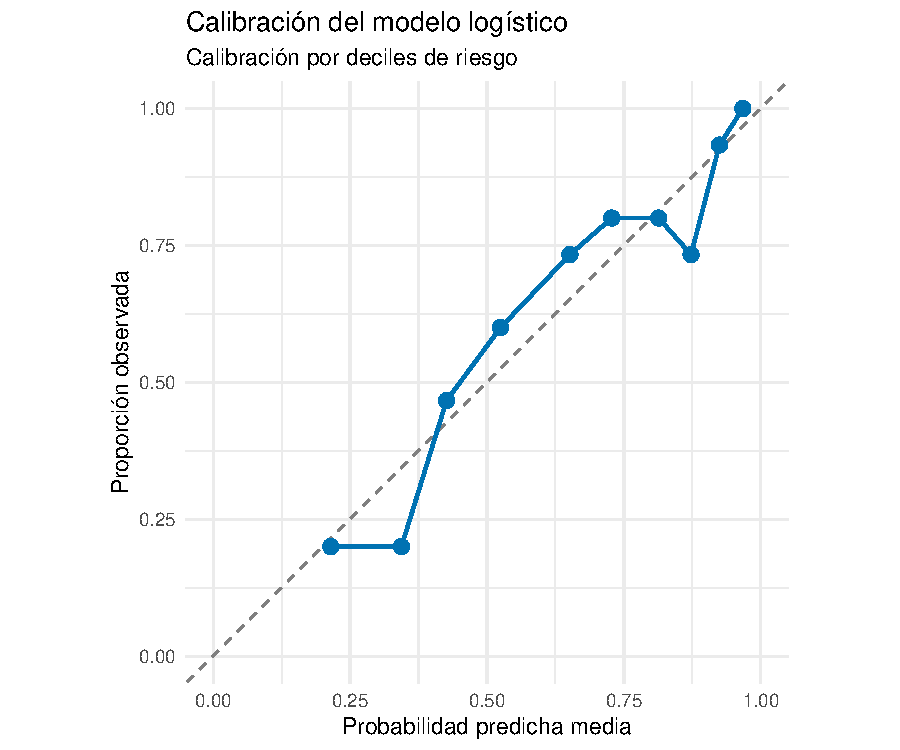
\includegraphics[width=0.7\linewidth,height=\textheight,keepaspectratio,alt={Gráfico que compara la probabilidad predicha media con la proporción observada de problemas respiratorios.}]{02-Informe_2_files/figure-pdf/fig-grafico-calibracion-1.pdf}

}

\end{figure}%

\subsubsection{¿Existen observaciones muy influyentes o patrones no
explicados?}\label{existen-observaciones-muy-influyentes-o-patrones-no-explicados}

\subsubsection{Obtenga una predicción de la probabilidad de presentar
problemas respiratorios para una niña de 4 años que presenta un nivel de
6.5 μg/dL de plomo en la
sangre.}\label{obtenga-una-predicciuxf3n-de-la-probabilidad-de-presentar-problemas-respiratorios-para-una-niuxf1a-de-4-auxf1os-que-presenta-un-nivel-de-6.5-ux3bcgdl-de-plomo-en-la-sangre.}

\section{Regresión Poisson}\label{regresiuxf3n-poisson}

\subsection{Modelo de regresión Poisson con variables Edad, Sexo y
Pb.}\label{modelo-de-regresiuxf3n-poisson-con-variables-edad-sexo-y-pb.}

\subsubsection{Cada una de las variables, ¿es estadísticamente
significativa al
10\%?}\label{cada-una-de-las-variables-es-estaduxedsticamente-significativa-al-10}

\subsubsection{¿Cuál es el exp(beta) asociado al Pb?
Interprete.}\label{cuuxe1l-es-el-expbeta-asociado-al-pb-interprete.}

\subsection{Incorpore el factor ``comuna'' al modelo Poisson
previo.}\label{incorpore-el-factor-comuna-al-modelo-poisson-previo.}

\subsubsection{¿Qué variable(s) cambia de significancia? ¿Qué
implica?}\label{quuxe9-variables-cambia-de-significancia-quuxe9-implica}

\subsubsection{¿Cuál es el exp(beta) asociado a sexo? ¿Cuál es la
referencia?}\label{cuuxe1l-es-el-expbeta-asociado-a-sexo-cuuxe1l-es-la-referencia}

\subsection{¿Existe sobredispersión? Si la respuesta es positiva,
estímela. Finalmente. obtenga la predicción de la frecuencia de
episodios respiratorios para un niño de 5 años que presenta un nivel de
5.5 μg/dL plomo en la
sangre.}\label{existe-sobredispersiuxf3n-si-la-respuesta-es-positiva-estuxedmela.-finalmente.-obtenga-la-predicciuxf3n-de-la-frecuencia-de-episodios-respiratorios-para-un-niuxf1o-de-5-auxf1os-que-presenta-un-nivel-de-5.5-ux3bcgdl-plomo-en-la-sangre.}




\end{document}
